\section{Optimized Grid Model}
\setlength{\parindent}{10ex}
%Purpose of this section is to identify the optimized grid structure.
%I need to check with Hoque to identify what I should and shouldnt include
%I need to consider rewording this and restructuring to manage the correctness for example etc.
The Optimized Grid Model is a structure devised for project to leverage locally effective models.
This model is built upon the idea that there is not a optimal single model for predicting all of the worlds bathymetry.
It leverages several different models to predict bathymetry in a area by recording the best preforming models across a grid of the world.
This allows the model to use the optimal model for predicting bathymetry.

%Give the background for the idea in this section!
\subsection{Grid Optimizing Background}
According to the "No Free Lunch Theorem" \cite{wolpert1997no}, there is no optimal model to solve all problems.
For machine learning this therom esspicially holds true.
To append onto the theorm, there is not a single model that will optimally predict the entire globes bathymetry.
A model that preforms well in a area of the pacific may not preform well in the atlantic.
This notion is intuitive as Earth's environments change across lattitude so will the features for prediction.
This was observed in the classification section of this work where each classifier varied in preformance by depth.

\par
There is potentially a configuration where each model has an optimal coverage of the earth.
This coverage should be designated to maximize accurate predictions.
Therefore, a proof of concept for this model will be to divide the Earth into coverages and test a set of models against each.
This will prove that a optimal set of coverages for a model does exsist, and that localizing these models will yield benefit for predictions.

%In this section I am defining what the Grid optimization is and why it matters.
%There may be a better name for this?? Who knows really...
\subsection{Grid Optimizing}
This idea was implemented by partioning the world into coverages.
These coverages represent an area of the Earth.
For this project, I trained a set of classification models on each coverage to predict bathymetry.
The model that most accuratly predicted bathymetry was then recorded and stored into a data structure.
This structure is a simple map of a bounding boxs and models.

\begin{figure}[h]
    \centering
    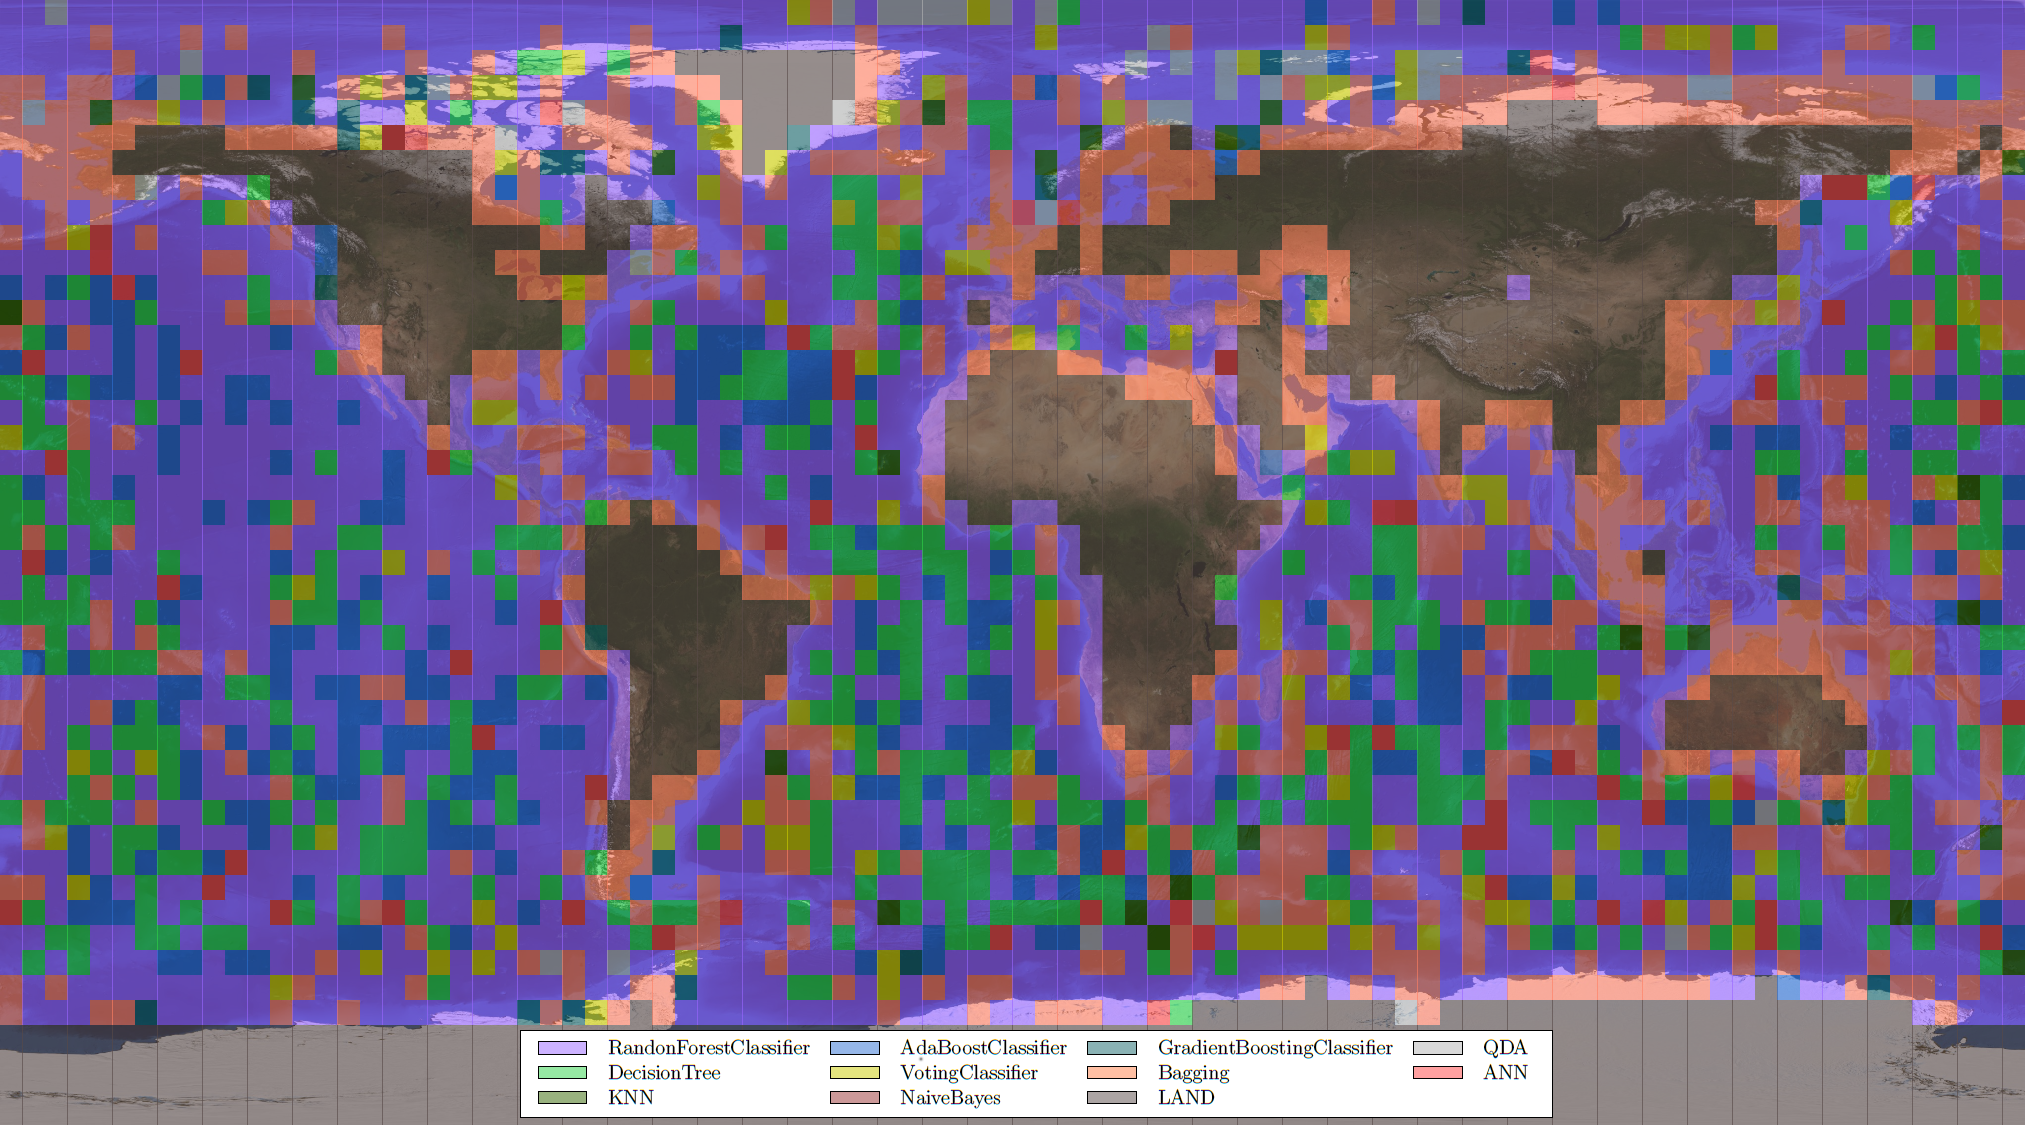
\includegraphics{optgriddraft.png}
    \caption{Graphic Showing the World Coverages and Successful Models}
    \label{fig:coveragegrid}
\end{figure}
%This is where I define what happens after the appropriate coverages have been found.
\par
The result of this "grid search" is a ensemble that selects the optimal model for predicting in a coverage.
Each model is trained on select portions of the world and validated.
This trained model is then persisted and stored for use in predictions.
The optimized grid model references the optimized grid structure then injects the best model for that coverage.

\par
In theory, this injection will allow each model to preform to its optimum.
Each coverage highlights distinct chracteristics that preform better for a certain estimator.
\ref{fig:coveragegrid} is a graphic representing where each model preformed best.
There are several patterns that can be gleaned from \ref{fig:coveragegrid}. 
There seems to be consistencies with depth, along fault lines, and potentially sediment coposition. 
% Reconsider this sentence....


\subsection{Results and Metrics}
%The world wide ETOPO bathymetry dataset \cite{national1988etopo} at two minute resolution is used for valadation and metrics.
%This dataset is treated as the ground truth for all predictions.
%During the experiment, a one third holdout was used for validation in some cases.
%For finding the optimum model for a coverage a 10 fold cross validation was utilized.

%Include metrics information here.... possibly graphs and a list of scores? I dont really know.

%I dont like how I worded this whole section...
%The idea here is that I want to say "Hey, these people did this research and found the their regression model preforms poorly for predicting seamounts espicially after 500m.
%I clearly noticed a similar trend, but saw better preformance from some models than others. 
%This research is to identify those coverages and then use those results to build a super classifier.
%These metrics are important for identifying where the models preform well. 
\par
A confusion matrix is generated for each model as a metric tool.
Balanced accuracy, precision, recall, F1 score, and support are also recorded for metrics.
These metrics give a measurement of the effectiveness for a model in a coverage.
%Extending off the research preformed in \cite{jena2012prediction} these metrics allow the selection of the best preforming model.

%Maybe here I can have a table show casing the preformance of models or possibly statistics about the coverages??
%It will be intersting to see what has preformed better across the globe
%Also is intersting to see which models have preformed best overall.
